\documentclass[10pt]{beamer}
\usepackage[latin1]{inputenc}
\usepackage{amsmath}
\usepackage{amsfonts}
\usepackage{amssymb}
\usepackage{graphicx} 
\usepackage{subfigure}
\usepackage{float}
\usepackage{hyperref}
\usepackage{color}

%%%%%%%%%%%%%%%%%%%%%%%
\usepackage{cite}
%\usepackage{algorithmic}
\usepackage{array}
\usepackage{mdwmath}
\usepackage{mdwtab}
\usepackage{eqparbox}
\usepackage{graphicx}
\usepackage[]{subfigure}
\usepackage{url}
\usepackage[algoruled,vlined,linesnumbered]{algorithm2e}

%%%%%%%%%%%%%%%%%%%%%%%
%\usecolortheme[RGB={0,255,0}]{structure} 
\usetheme{Warsaw}
\setbeamertemplate{subsection in head/foot shaded}[default][20] 
\logo{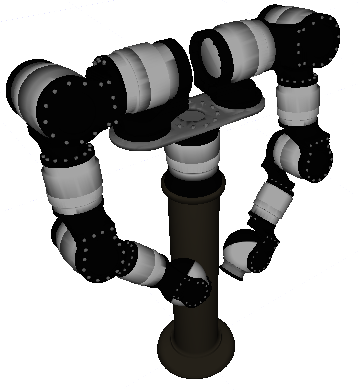
\includegraphics[height=2.0cm]{images/small_StartRobot.png}} 


% *********************************************************
% Math characters shortcuts
\newcommand{\J}{\ensuremath{J}}
\newcommand{\Jps}{\ensuremath{J^{\dagger}}}
\newcommand{\dx}{\ensuremath{\dot{x}}}
\newcommand{\dq}{\ensuremath{\dot{q}}}
\newcommand{\q}{\ensuremath{q}}
\newcommand{\JsPath}{\ensuremath{\mathcal{Q}}}
\newcommand{\WsPath}{\ensuremath{\mathcal{P}}} % Workspace path
\newcommand{\Wsp}{\ensuremath{p}} % Workspace point
\newcommand{\nsb}{\ensuremath{\hat{e}}} % Nullspace basis
\newcommand{\nsc}{\ensuremath{w}}  % Nullspace coefficients
\newcommand{\nsS}{\ensuremath{\mathcal{NS}}}  % Nullspace Set - vector of queues
\newcommand{\nss}{\ensuremath{ns}}  % Nullspace element single queue



\author{Ana Huam\'{a}n Quispe and Mike Stilman}
\title{ Deterministic Motion Planning for Redundant Robots along End-Effector Paths }

\begin{document}
\maketitle

% ---------------------------------
% Research problem
\begin{frame}
\frametitle{Problem Statement}

\begin{center}
\begin{Large}
{\color{blue} Motion Planning along End-Effector Paths \\ for redundant manipulators \\ (MPEP) }
\end{Large}
\end{center}

\end{frame}


% ---------------------------------
% Research problem
\begin{frame}
\frametitle{Example}

\begin{center}
\begin{normalsize}
{\color{blue} Given an End-Effector path to follow find a corresponding path in configuration space}
\end{normalsize}
\end{center}

\begin{figure}[]
		\centering
		  \subfigure[Manipulator]{
		   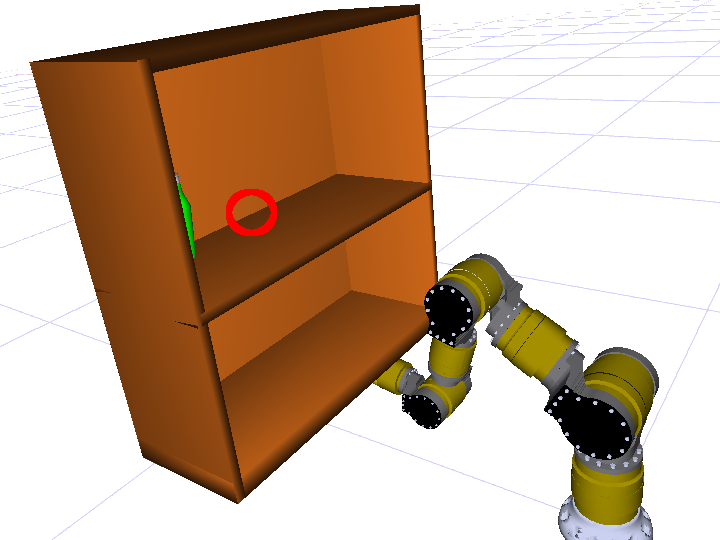
\includegraphics[width=0.3\textwidth]{images/Experiment_LWA3_Path_2_StartTarget_720x540.png} 
		   \label{fig:IntroExample_Manip}
          }
          \subfigure[End-Effector Path]{
	       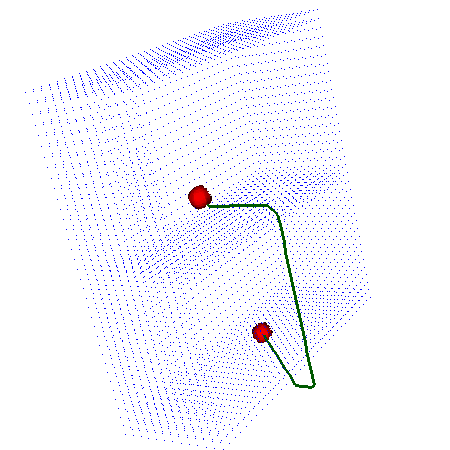
\includegraphics[width=0.3\textwidth]{images/Experiment_LWA3_WSPath_2_450x450.png} 	
	       \label{fig:IntroExample_WS}
          }
          \caption{Example}
          \label{fig:IntroExample}
\end{figure}


\end{frame}

% ---------------------------------
% Research problem
\begin{frame}
\frametitle{Example}

\begin{center}
	\begin{normalsize}
	{\color{blue} Potential problems}
	\end{normalsize}

	\begin{itemize}
		\item{ Many possible configurations at each waypoint! }
		\item{ How do we choose? (and avoid potential local minima) }
	\end{itemize}
\end{center}

\begin{figure}[]
		\centering
		  \subfigure[1 time step]{
		   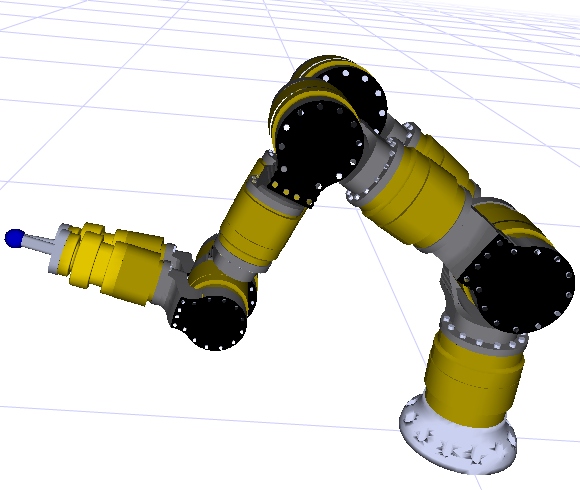
\includegraphics[width=0.3\textwidth]{images/singleNS_illustration1.png} 
		   \label{fig:IntroExample_OneStep}
          }
          \subfigure[n time steps]{
	       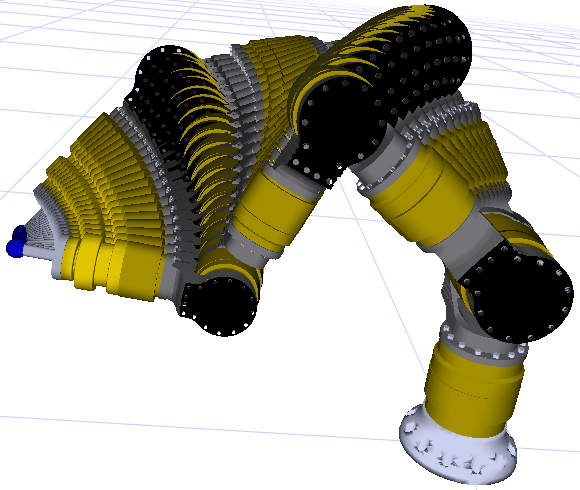
\includegraphics[width=0.3\textwidth]{images/completeNS_illustration1.png} 	
	       \label{fig:IntroExample_MultipleSteps}
          }
          \caption{Example}
          \label{fig:IntroSteps}
\end{figure}


\end{frame}

% ----------------------------------
% Approach
\begin{frame}
\frametitle{Our Approach I}
\begin{center}
	\begin{normalsize}
		{\color{blue} \underline{Background} }
	\end{normalsize}
\end{center}
% Items
\begin{itemize}
% Forward Kinematics Item
\item{ {\color{blue}Forward kinematics:}
	\begin{equation}
		x = f(\q)
		\label{eq:FK}
	\end{equation}
	
and its differential version is expressed as:
	\begin{equation}
		\dot{x} = \J \dq
		\label{eq:Diff_FK}
	\end{equation}	}
% Inverse Kinematics Item	
\item{ {\color{blue}Inverse Kinematics:}
The solution to (\ref{eq:Diff_FK}) is normally expressed as:

	\begin{equation}
		\dq = \Jps \dx + (I - \Jps \J)\dq_{0}
		\label{eq:IK_GeneralSol}
	\end{equation} }
\end{itemize}

\end{frame}

%%%%%%%%%%%%%%%%%%%%%%%%%%%%%%%%%%%%%
% Our Approach II
\begin{frame}
\frametitle{Our Approach II}

\begin{center}
	\begin{normalsize}
		{\color{blue} \underline{Our representation}}
	\end{normalsize}
\end{center}

\begin{itemize}
% Our formula
\item{ We express Eq. (\ref{eq:IK_GeneralSol}) as:

	\begin{equation}
		\dq = \Jps \dx + \displaystyle \sum_{i=1}^{n-m} \nsc_{i}\nsb_{i}
		\label{eq:Proposed_Eq1}
	\end{equation}

	where:
	\begin{itemize}
		\item{ $\nsb_{i}$: Normalized basis of the Jacobian nullspace}
		\item{$\nsc_{i}$: Coefficients of each $\nsb_{i}$}
	\end{itemize} }
% Why is this good?	
\item{Why is this good? Because we can discretize the nullspace ($\nsb_{i}$) and search through it!}
\end{itemize}
\end{frame}


%%%%%%%%%%%%%%%%%%%%%%%%%%%%%%%%%%%%%
% Our Approach III
\begin{frame}
\frametitle{Our Approach II}

\begin{center}
	\begin{normalsize}
		{\color{blue} \underline{How do we choose the weights?}}
	\end{normalsize}
\end{center}

\begin{itemize}
% Weights
\item{ We use heuristics functions (as proposed in previous work by Kapoor et al (1998):) 
	\begin{itemize}
		\item{ {\color{blue}Joint Range Availability measurement (JRA) }
			\begin{equation}
				JRA(\q)=  \displaystyle \sum_{i=1}^{n} \dfrac{ \q_{i} - {\bar{\q}}_{i} }{ {\q_{i}}_{Max} - {\q_{i}}_{Min} }
			\end{equation} }

		\item{ {\color{blue}Joint Velocity Measurement (JVM)}		
			\begin{equation}
				JVM(\q)=  \displaystyle \sum_{i=1}^{n} ( \q_{i} - {\q}_{i}_{previous} )
			\end{equation}		
		}

	\end{itemize}
}
\end{itemize}
\end{frame}

%%%%%%%%%%%%%%%%%%%%%%%%%%%%%%%%%%%%%
\begin{frame}
\frametitle{Our Algorithm}

\begin{figure}[h] 
   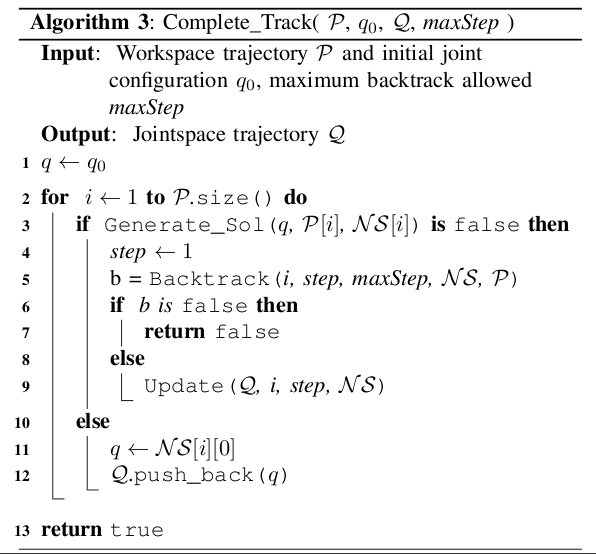
\includegraphics[scale=0.3]{images/algorithmCompleteTrack.png} 
   \label{fig:Algorithm}
   %\caption{Main function}
\end{figure}

\begin{scriptsize}
\textit{A. Huam\'{a}n Quispe and M. Stilman \\}
\textit{Deterministic Motion Planning for Redundant Robots along End-Effector Paths \\}
\textit{Proceedings of 2012 IEEE-RAS International Conference on Humanoid Robots}
\end{scriptsize}

\end{frame}

\end{document}